%-----------------------------------------------------------------------------
%	PACKAGES AND DOCUMENT CONFIGURATIONS
%-----------------------------------------------------------------------------

\documentclass{article}

\usepackage{graphicx} % Required for the inclusion of images
\usepackage{natbib} % Required to change bibliography style to APA
\usepackage{amsmath} % Required for some math elements
\usepackage{amssymb}
\usepackage{grffile}
\usepackage[export]{adjustbox}
\usepackage{subcaption}
\usepackage{float}
\usepackage{listings}
\usepackage[margin=1.0in]{geometry}
\usepackage{tikz}
\usepackage{enumitem}
\usepackage{scrextend}
\usepackage{siunitx}
\usepackage{minted}

\usetikzlibrary{shapes.geometric, arrows}
\tikzstyle{startstop} = [rectangle, rounded corners, minimum width=1cm, minimum height=1cm,text centered, draw=black, fill=white!30]
\tikzstyle{process} = [rectangle, minimum width=1.5cm, minimum height=1cm, text centered, draw=black, fill=white!30]
\tikzstyle{arrow} = [thick,<->,>=stealth]

\renewcommand{\baselinestretch}{1.5}
\setlength\parindent{0pt} % Removes all indentation from paragraphs

%-----------------------------------------------------------------------------
%	DOCUMENT INFORMATION
%-----------------------------------------------------------------------------

\title{ECE 547 Homework 6} % Title

\author{Yang \textsc{Wang}}  % Author name

\date{\today} % Date for the report

\renewcommand{\theenumi}{\alph{enumi}} % use letters for list items

\begin{document}

\maketitle % Insert the title, author and date

%-----------------------------------------------------------------------------
%	Problems
%-----------------------------------------------------------------------------

\section*{Problem 1}
	\begin{enumerate}
		\item The total number of ways to put $n$ balls into $M$ boxes is simply
			asking us how many ways to arrange $(n + M - 1)$ objects. Hence, this can
			be simply written as;
			\begin{align*}
				C(M) = \frac{(n+M-1)!}{n!(M-1)!} = \binom{n+M-1}{n}
			\end{align*}
		\item We need to check for the result when $n = 3$ and $M = 4$. Intuitively,
			say we have 3 balls and 4 boxes. How many ways can we arrange the balls
			to these 4 boxes? Let us denote a sequence $abcd$ where:
			\begin{align*}
				a &= \text{ number of balls in box 1} \\
				b &= \text{ number of balls in box 2} \\
				c &= \text{ number of balls in box 3} \\
				d &= \text{ number of balls in box 4}
			\end{align*}
			Hence, we can have 0003, 0030, 0300, 3000, 0012, 0120, 1200, 1020, 1002,
			0102, 0021, 0201, 0210, 2010, 2100, 2001, 0111, 1011, 1110, 1101, a total
			of 20 ways to arrange the balls. From the result in part (a), we can
			obtain:
			\begin{align*}
				C(4) &= \frac{(3+4-1)!}{3!(4-1)!} = 20
			\end{align*}
			Therefore, we verified the result in part (a).
		\item THe total number of combinations that results in 0 packets in queue
			is the number of ways to put $n$ balls into $()$ boxes. Hence, from the
			result in part (a):
			\begin{align*}
				C(M-1) &= \frac{(n+(M-1)-1)!}{n!(M-1-1)!} = \binom{n+M-2}{n}
			\end{align*}
			Therefore, we can find the probability that a queue is empty:
			\begin{align*}
				P_{0} &= \frac{C(M-1)}{C(M)} \\
					&= \frac{\frac{(n+M-2)!}{n!(M-2)!}}{\frac{(n+M-1)!}{n!(M-1)!}} \\
					&= \frac{M-1}{n+M-1}
			\end{align*}
			Hence, the throughput can be calculated as:
			\begin{align*}
				\mu(n) &= \mu (1-P_{0}) \\
				&= \frac{\mu \cdot n}{n+M-1}
			\end{align*}
	\end{enumerate}

\section*{Problem 2}
	\begin{enumerate}
		\item Based on the Norton's Equivalent network diagram in the homework, we
			can draw the state transition diagram as in Figure 1.
			\vspace{40mm}

			We can write the balance equations based on the state transition diagram:
			\begin{gather*}
				P_{0} \lambda(N) = \mu P_{1} \implies P_{1} = P_{0} \frac{\lambda(N)}{\mu} \\
				P_{1} \lambda(N-1) = \mu P_{2} \implies P_{2} = P_{0} \frac{\lambda(N)}{\mu} \frac{\lambda(N-1)}{\mu} \\
				\ldots \\
				\implies P_{n} = \frac{\prod\limits_{i=1}^{n} \lambda(N-(i-1))}{\mu^{n}} P_{0}
			\end{gather*}
			We can then find $P_{0}$ by normalizing the probability of number of
			packets $P_{n}$:
			\begin{gather*}
				\sum\limits_{n=0}^{N} P_{n} = 1 \\
				P_{0} + P_{0} \sum\limits_{n=1}^{N} \frac{\prod\limits_{i=1}^{n} \lambda(N-(i-1))}{\mu^{n}} = 1 \\
				\implies P_{0} = \frac{1}{1 + \sum\limits_{n=1}^{N} \frac{\prod\limits_{i=1}^{n} \lambda(N-(i-1))}{\mu^{n}}}
			\end{gather*}
			With $P_{0}$, it enables us to find $P_{n}$ and the average throughput,
			the average time delay:
			\begin{gather*}
				\mu(k) = \mu(1 - P_{0}) \\
				E[n] = \sum\limits_{n=0}^{N} nP_{n} \\
				E[T] = \frac{E[n]}{\gamma} = \frac{E[n]}{\mu(k)} \text{ by Little's Law}
			\end{gather*}
		\item Solving $\lambda(k)$ requires us to short the upper half the closed
			queue network. The shorted network diagram is shown in Figure 2.
			\begin{figure}[!hbt]
				\centering
				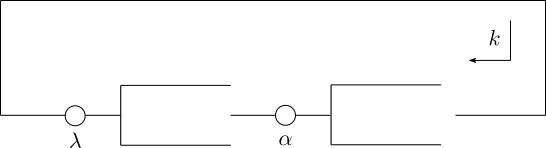
\includegraphics[width=0.8\linewidth]{hw6_2_norton.png}
			\end{figure}

			We can then draw the state transition diagram based on the shorted
			network.
			\vspace{40mm}
			
			By writing the balance equations,
			\begin{gather*}
				P_{0} \lambda = P_{1} \alpha \implies P_{1} = \frac{\lambda}{\alpha} P_{0} \\
				P_{1} \lambda = P_{2} \alpha \implies P_{2} = \left(\frac{\lambda}{\alpha}\right)^2 P_{1} \\
				\ldots
			\end{gather*}
			we find that $P_{n}=\left(\frac{\lambda}{\alpha}\right)^n P_{0}$.
			By normalizing $P_{n}$:
			\begin{gather*}
				\sum\limits_{n=0}^{k} \left(\frac{\lambda}{\alpha}\right)^n P_{0} = 1 \\
				P_{0} \sum\limits_{n=0}^{k} \left(\frac{\lambda}{\alpha}\right)^n = 1 \\
				P_{0} = \frac{1}{\frac{1-(\frac{\lambda}{\alpha})^{k+1}}{1-\frac{\lambda}{\alpha}}} \\
				\implies P_{0} = \frac{1-\frac{\lambda}{\alpha}}{1-(\frac{\lambda}{\alpha})^{k+1}}
			\end{gather*}
			Therefore, we can get $\lambda(k)=\lambda(1-P_{0})$.
	\end{enumerate}

\section*{Problem 3}
	\begin{enumerate}
		\item Let $X$ be the number of times of that a typical packet needs to be
			(re)transmitted. Then we can have:
			\begin{align*}
				P({X=1}) &= 1-p \\
				P({X=2}) &= p^{1}(1-p) \\
				P({X=3}) &= p^{2}(1-p) \\
				&\ldots \\
				\implies P({X=n}) &= p^{n-1}(1-p)
			\end{align*}
			Then, the expected value of $X$, $E[X]$ can be written as:
			\begin{align*}
				E[X] &= \sum\limits_{n=1}^{\infty} np^{n-1}(1-p) \\
				&= \frac{1}{1-p}
			\end{align*}
		\item We would first try writing down the state transition diagram as shown
			in Figure 4. The station transition diagram resembles an M/M/1 queue with
			service rate $\frac{1-p}{C}$.
			\vspace{40mm}
			
			Based on the state transition diagram, we can derive the balance
			equations:
			\begin{gather*}
				P_{0} \lambda = P_{1} \frac{1-p}{C} \implies P_{1} = \frac{\lambda}{\frac{1-p}{C}} P_{0} \\
				P_{1} \lambda = P_{2} \frac{1-p}{C} \implies P_{2} = \left(\frac{\lambda}{\frac{1-p}{C}}\right)^{2} P_{0} \\
				\implies P_{n} = \left(\frac{\lambda}{\frac{1-p}{C}}\right)^{n} P_{0}
			\end{gather*}
			By normalizing $P_{n}$, we can easily find that $P_{0}=1-\frac{\lambda}{\frac{1-p}{C}}$.
			Hence, $P_{n}=\left(\frac{\lambda}{\frac{1-p}{C}}\right)^{n} \left(1-\frac{\lambda}{\frac{1-p}{C}}\right)$.
			We can further denote $\rho=\frac{\lambda}{\frac{1-p}{C}}$.
			Since the network resembles an M/M/1 queue, we can obtain:
			\begin{align*}
				E[n] &= \frac{\rho}{1-\rho} \\
				E[T] &= \frac{E[n]}{\lambda} \text{ (Little's Law)}
			\end{align*}
	\end{enumerate}

\section*{Problem 4}
	(I am not sure about this problem.)

	From page 233 of Schwartz textbook, the networkwide expected delay can be
	calculated as the following:
	\begin{align*}
		E[T] = \frac{1}{\gamma} \sum\limits_{i=1}^{M} \frac{\lambda_{i}}{\mu_{i} - \lambda_{i}}
	\end{align*}
	Hence, for each node, the service rate $\mu_{i} = \mu p$. On the other
	hand, the arrival rate at each node is $\lambda_{i} = \mu p + \lambda$.
	Therefore, the networkwide expected delay is:
	\begin{align*}
		E[T] &= \frac{1}{3\lambda} \cdot 4 \cdot \frac{\mu p + \lambda}{\mu p} \\
		&= \frac{4}{3\lambda} \left( 1 + \frac{\lambda}{\mu p} \right) \\
		&= \frac{4}{3\lambda} + \frac{4}{3} \cdot \frac{1}{\mu p}
	\end{align*}

\end{document}
